% This is samplepaper.tex, a sample chapter demonstrating the
% LLNCS macro package for Springer Computer Science proceedings;
% Version 2.20 of 2017/10/04
%
\documentclass[runningheads]{llncs}
%
\usepackage{graphicx}
\usepackage{listings}
\usepackage{color}

\definecolor{dkgreen}{rgb}{0,0.6,0}
\definecolor{gray}{rgb}{0.5,0.5,0.5}
\definecolor{mauve}{rgb}{0.58,0,0.82}

    
\lstset{frame=tb,
  language=Java,
  aboveskip=3mm,
  belowskip=3mm,
  showstringspaces=false,
  columns=flexible,
  basicstyle={\small\ttfamily},
  numbers=none,
  numberstyle=\tiny\color{gray},
  keywordstyle=\color{blue},
  commentstyle=\color{dkgreen},
  stringstyle=\color{mauve},
  breaklines=true,
  breakatwhitespace=true,
  tabsize=3
}

% Used for displaying a sample figure. If possible, figure files should
% be included in EPS format.
%
% If you use the hyperref package, please uncomment the following line
% to display URLs in blue roman font according to Springer's eBook style:
% \renewcommand\UrlFont{\color{blue}\rmfamily}
\renewcommand\refname{Bibliografia}
\begin{document}
%
\title{Chess-Num Puzzles Solver}
\author{Diogo Samuel Gonçalves Fernandes \and
Paulo Jorge Salgado Marinho Ribeiro}
\authorrunning{Diogo Fernandes \and
Paulo Ribeiro}

\institute{Faculdade de Engenharia da Universidade do Porto, \\
Rua Dr. Roberto Frias, 4200-465, Porto, Portugal, \\
FEUP-PLOG, Turma 3MIEIC06, Grupo Chess-Num\textunderscore 2\\
\email{up201806250@fe.up.pt}\\
\email{up201806505@fe.up.pt}}
%Grupo e turma
%\url{$https://sigarra.up.pt/feup/pt/web_page.inicial$}
%
\maketitle
\begin{abstract}
Estre projeto foi desenvolvido no âmbito da unidade curricular \emph{Programação em Lógica} e consiste na resolução de um problema
de decisão, recorrendo ao uso de restrições em PROLOG através do uso da biblioteca CLPFD. O objetivo do nosso trabalho é resolver
os puzzle de Xadrez de forma a que todas as casas numeradas com um número N no tabuleiro sejam atacadas N vezes.

\keywords{Programação em Lógica  \and Prolog \and Restrições \and clpfd \and SICStus \and Problemas de Otimização \and Problemas de Decisão.}
\end{abstract}

\section{Introdução}
A Programação em Lógica com Restrições trata-se de uma classe de linguagens de programação, que combina a declaratividade característica da programação em lógica
e a eficiência da resolução de restrições. 

As suas principais aplicações baseiam-se na resolução de problemas de pesquisa ou otimização combinatória, 
tal como problemas de escalonamento, geração de horários, alocação de recursos, gestão de produção, entre outros.

Dada a sua distinção e eficiência, a Programação em Lógica com Restrições tem diversas aplicações industriais e comerciais na atualidade, 
destacando-se a sua utilização na Renault, para planeamento de produção a curto prazo, na Nokia, para configuração de software para telemóveis 
e na Siemens, para verificação de circuitos \cite{slides1}.

Neste trabalho, aplicaremos estas capacidades na resolução de puzzles Chess-Num, que consistem na colocação de uma peça de Xadrez de cada tipo [Peão, Torre, Bispo, Cavalo, Rainha, Rei] 
num tabuleiro com casas numeradas, de modo a que todas as casas numeradas sejam atacadas N vezes, sendo N o número apresentado em cada uma dessas casas. 
Alguns exemplos de puzzles deste tipo podem ser observados no site que contém as regras deste puzzle \cite{chessnum}.

\newpage
Este relatório procura explicar a nossa abordagem do problema de forma aprofundada e organizada nos seguintes tópicos:

\begin{itemize}
    \item \textbf{Descrição do Problema}: Descrição do problema detalhadamente e restrições envolvidas.
    \item \textbf{Abordagem}: Implementação do problema, com enumeração das variáveis de decisão e dos seus domínios.
    \item \textbf{Visualização da Solução}: Exploração dos predicados que permitem a visualização do problema resolvido e respetivas imagens exemplificativas.
    \item \textbf{Experiências e Resultados}: Análise dimensional do problema, para distintas quantidades de células numeradas e diferentes tamanhos do tabuleiro. 
    \item \textbf{Conclusões e Trabalho Futuro}: Conclusões que retiramos deste projeto, com base nos resultados obtidos, e possíveis formas de melhorar o trabalho desenvolvido
    \item \textbf{Referências}: com enumeração das várias fontes bibliográficas que utilizamos para a procura de conhecimento
    \item \textbf{Anexos}: que contêm imagens explicativas de alguma secção do relatório, e imagens exemplificativas do programa em execução
\end{itemize}

\section{Descrição do Problema}
O nosso tema aborda um problema de decisão, que consiste na resolução de um tipo de puzzle envolvendo peças de xadrez. 
No tabuleiro vão existir casas numeradas, de 1 a 6.
 A solução consiste em colocar uma peça de cada tipo [Peão, Cavalo, Rei, Torre, Bispo, Rainha] no tabuleiro, de modo a que cada uma destas casas seja
atacada N vezes, sendo N o número presente na casa. O ataque das peças é identico ao do jogo Xadrez \cite{chessmove}:
\begin{itemize}
    \item  O peão ataca na diagonal, para cima, atacando duas casas distintas.
    \item  O cavalo ataca em L, atacando oito casas distintas. 
    \item  O bispo ataca todas as diagonais.
    \item  A torre ataca todas as verticais e horizontais.
    \item  O rei ataca todas as casas à sua volta, num alcance de uma casa, atacando oito casas distintas.
    \item  A rainha todas as diagonais, verticais e horizontais.
\end{itemize}

É importante referir ainda que ao contrário do jogo de xadrez, é possível colocar os peões 
na primeira e última linha. Não é possível colocar duas peças na mesma casa, nem numa casa que tenha numeração.
Deve-se ter também em conta que tanto a torre como o bispo e a rainha não atacam uma dada casa se existir alguma peça entre eles, bloqueando o caminho.

\newpage
\section{Abordagem ao Problema}
O nosso problema trata-se de um problema de satisfação de restrições (PSR), e pode ser modelizado por um conjunto de variáveis que representam diferentes aspetos do problema, os seus respetivos domínios, e restrições que limitam os valores que estas podem tomar dentro dos seus domínios.
A solução consiste na atribuição de valores às variáveis de modo a que todas as restrições sejam satisfeitas. No nosso caso, a solução consiste em encontrar uma disposição de peças de tal forma a que cada casa numerada seja atacada um número de vezes igual àquele que contém.

Para a resolução deste problema utilizando a \emph{CLPFD} em \emph{PROLOG} foi utilizada uma lista de listas para representar a
o tabuleiro de xadrez.

\subsection{Variáveis de Decisão}
    A solução ao problema encontra-se nas seguintes variáveis listadas abaixo. As variáveis \emph{piece}X, \emph{piece}Y 
    representam os possíveis valores da linha e coluna das peças de xadrez \emph{piece}.
    
    \begin{itemize}
        \item PawnX, PawnY
        \item KnightX, KnightY
        \item KingX, KingY
        \item RookX, RookY
        \item BishopX, BishopY
        \item QueenX, QueenY
    \end{itemize}
    
    Estas variáveis de decisão são reunidas numa lista, Positions, que será depois utilizada ao efetuar o labeling.
    Cada par destas variáveis corresponde à posição de uma dada peça no tabuleiro, sendo o primeiro elemento do par a linha onde a peça se encontra, e o segundo elemento a coluna.
    Assim, as variáveis pertencem ao domínio [1, N] em que N é o tamanho do tabuleiro. Estes são os valores possíveis que a linha/coluna pode assumir no tabuleiro.
    
\subsection{Restrições}
    As restrições a definir devem garantir a solução do problema, isto é, que para cada casa numerada, esta seja atacada N vezes, sendo N o número que contém. Para isto, foi necessário definir a zona de ataque de cada tipo de peça.
    Na secção de código dos anexos, é possível observar estes predicados para cada tipo de peça (Peão, Cavalo, Rei, Torre, Bispo, Rainha), nos pontos 1.2, 1.3, 1.4, 1.5, 1.6, e 1.7, respetivamente para cada tipo de peça. Em todos usamos restrições materializadas (reified), para que a variável Attack ficasse definida com o valor 1 no caso de as restrições que verificam se a célula é atacada por uma dada peça serem cumpridas, e 0 caso contrário.
    Assim, após serem chamados todos os seis predicados, basta somar os seis ataques retornados nos predicados de cada peça, e o resultado será o número de vezes que a casa está atacada, que terá de ser igual ao número que essa casa contém.
    Isto tudo é realizado no predicado cell\textunderscore attacks, que verifica estas condições para uma dada casa numerada (secção do código no anexos, ponto 1.1). A verificação destas restrições para todas as casas numeradas é realizada no predicado principal, solve, com recurso ao predicado maplist, que aplica este predicado cell\textunderscore attacks a cada uma das casas numeradas, que foram reunidas numa lista, no início do programa, numa chamada ao predicado getCellsNumber.
    É necessário ter em conta também os possíveis bloqueios de peças, nos casos da Torre, Bispo e Rainha. Para isto, criamos um predicado nothing\textunderscore between, que verifica se não há nenhuma peça a bloquear o caminho entre a Torre/Rainha e a casa numerada, na horizontal e vertical.
    Da mesma forma, foi necessário criar o predicado nothing\textunderscore between\textunderscore diagonal, que verifica se não há nenhuma peça a bloquear o caminho entre Bispo/Rainha e a casa numerada, nas diagonais.
    Estas duas funções que analisam os bloqueios podem também ser observadas nos anexos, na secção do código, pontos 1.8 e 1.9.

\section{Visualização da Solução}

Para uma melhor compreensão das soluções encontradas, decidimos implementar duas formas de apresentação das soluções:
\begin{itemize}
    \item \textbf{Forma Escrita}:
    Apresenta-se no ecrã as posições de cada uma das seis peças, no formato [Linha, Coluna].
    Isto é efetuado pelo predicado show\textunderscore results, que recebe a lista das posições das peças e o número da peça a que a próxima posição corresponde. Trata-se de um ciclo simples, e recorre ao predicado piece, que recebe o número da peça e retorna o respetivo nome.
    Tanto a implementacão deste predicado como o seu funcionamento com o programa em execução podem ser visualizados nos anexos, na figura 4 e na secção de código, ponto 1.10.
    \item \textbf{Tabuleiro}:
    É apresentado um tabuleiro com as células numeradas e com as seis peças já colocadas conforme a solução encontrada, com uma respetiva legenda.
    Isto é efetuado pelo predicado display\textunderscore solution, que chama o predicado add\textunderscore pieces, responsável por substituir os valores das células dos tabuleiros contidos em Positions, pela peça de Xadrez correspondente. De seguida, é chamado o predicado display\textunderscore board, que representa visualmente o tabuleiro já preenchido. Um exemplo deste tipo de visualização pode ser observado na figura 3.
    Da mesma forma, é apresentado o tabuleiro do problema (apenas com as células numeradas) antes de se iniciar a procura da solução.
\end{itemize}

\newpage
\section{Experiências e Resultados}
\subsection{Análise Dimensional}
Para o estudo do comportamento do programa face à dimensão do problema, consideramos dois tipos de testes: 
\begin{itemize}
    \item Variação da dimensão do tabuleiro
    \item Variação do número de células numeradas.
\end{itemize}

É possível verificar os resultados para os testes do primeiro tipo na figura 1 dos anexos, sendo que testamos, para um mesmo número de casas numeradas, distintos tamanhos para os tabuleiros.
Conclui-se que  que o tempo de execução aumenta com a dimensão do tabuleiro, o que seria de esperar, uma vez que aumenta também o domínio das variáveis de decisão (é de 1 a N, sendo N o tamanho do tabuleiro, que é o valor mínimo e máximo que a Linha/Coluna da peça pode tomar, respetivamente), e portanto aumenta o número de testes efetuados pelas restrições.

Quando à variação do número de células numeradas, testamos para um mesmo tabuleiro (8x8), diferentes valores, o que pode ser verificado na figura 2 dos anexos.
Como seria também de esperar, o tempo de execução aumenta com o número de casas numeradas, uma vez que aumenta também o número de restrições a ter em consideração, e, consequentemente, o número de tentativas a serem efetuadas pelo programa.

\subsection{Estratégias de Pesquisa}

De modo a detetar possíveis melhorias no tempo de resolução dos problemas, foram testadas diversas combinações para as opções de pesquisa do labeling. 

Após realizar estes testes, chegamos à conclusão que no nosso caso a melhor combinação de opções do labeling seriam a anti\textunderscore first\textunderscore fail e
 a bisect.
A opção escolhida para a ordenação de variáveis (anti\textunderscore first\textunderscore fail) define que a próxima variável a ser escolhida na colocação 
das restrições é a variável mais à esquerda das que têm o maior domínio.
A complementá-la, a opção escolhida para a seleção de valores define que os valores de uma 
variável são decididos através de uma escolha binária entre X  \#$=<$ M e X  \#$>$ M, onde M 
é o ponto médio do domínio de X (média entre valores mínimo e máximo do domínio de X, 
com arredondamento para baixo).

\newpage
\section{Conclusões e Trabalho Futuro}

A realização deste trabalho permitiu a resolução de um problema através da utilização de restrições lógicas na linguagem PROLOG,
através da utilização do módulo CLPFD.
Durante a realização do mesmo foram encontradas diversas dificuldades, nomeadamente na elaboração dos ataques para a torre e para o bispo e rainha, devido aos possíveis bloqueios de peças que se encontrem entre estas peças e as casas numeradas.
Com o tempo, descobrimos solução para esta dificuldade, recorrendo a restrições materializadas.

Apesar de cumprir todos os requisitos pedidos no enunciado, há certos aspetos que poderiam ser melhorados futuramente, nomeadamente a questão da eficiência do programa, tendo em conta que o tempo de execução do programa
é elevado no caso de tabuleiros com um elevado número de casas numeradas.

Em suma, o projeto foi concluído com sucesso, tendo em conta que implementamos todos os requisitos do enunciado, e conseguimos ultrapassar todas as dificuldades que enfrentamos durante o seu desenvolvimento.
Implementamos também certas funcionalidades extra e interessantes, como a geração aleatória de tabuleiros, de diferentes dimensões, e com números distintos de casas numeradas. Para além disto, tornamos a interface de interação com o utilizador bastante simples e fácil de compreender,
com representação gráfica dos tabuleiros antes e após as soluções. Este projeto permitiu-nos aplicar o conhecimento obtido nas aulas teóricas e práticas da unidade curricular, e consolidá-lo para que possamos aplicá-lo em situações futuras.

%
% ---- Bibliography ----
%
% BibTeX users should specify bibliography style 'splncs04'.
% References will then be sorted and formatted in the correct style.
\newpage
\begin{thebibliography}{8}
\bibitem{slides1}
Daniel Castro Silva, Programação em Lógicacom Restrições [PowerPoint Slides], \url{https://moodle.up.pt/}

\bibitem{slides2}
Daniel Castro Silva, Programação em Lógica com Restrições no SICStus Prolog [PowerPoint Slides], \url{https://moodle.up.pt/}

\bibitem{chessnum}
Chess-Num Puzzles, \url{https://erich-friedman.github.io/puzzle/chessnum/}. Último acesso a 3
Jan 2021

\bibitem{chessmove}
Chess Pieces and How they move, \url{https://www.wholesalechess.com/pages/new-to-chess/pieces.html}. Último acesso a 3
Jan 2021

\end{thebibliography}

\newpage
\section{Anexos}
\subsection{Gráficos}
\begin{figure}
    \centering
    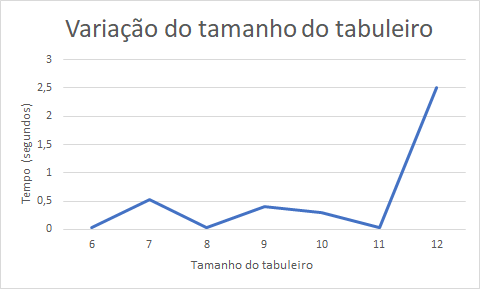
\includegraphics[scale=0.5]{./images/tamanhotabuleiro.png}
    \caption{Gráfico do tempo conforme o tamanho do tabuleiro} \label{fig1}
\end{figure}

\begin{figure}
    \centering
    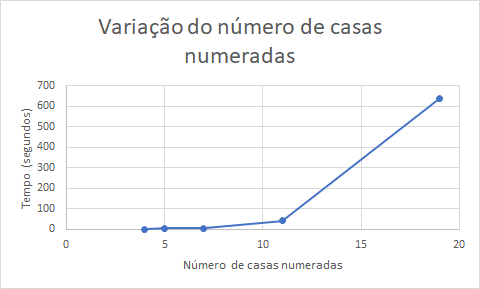
\includegraphics[scale=0.5]{./images/casasnumeradas.png}
    \caption{Gráfico do tempo conforme o número de casas numeradas} \label{fig2}
\end{figure}

\begin{figure}
    \centering
    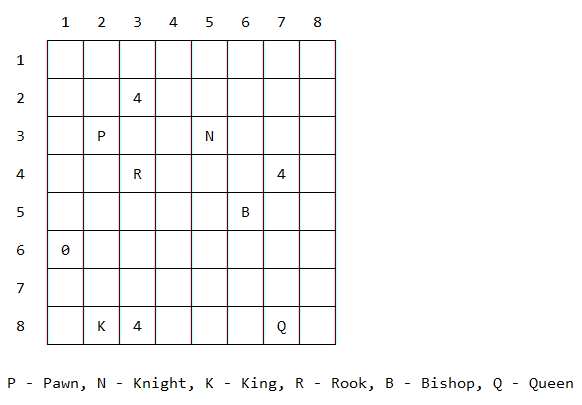
\includegraphics[scale=0.5]{./images/solution.png}
    \caption{Visualização gráfica} \label{fig2}
\end{figure}

\begin{figure}
    \centering
    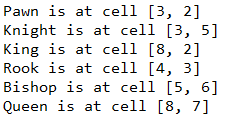
\includegraphics{./images/text.png}
    \caption{Visualização em texto} \label{fig2}
\end{figure}

\newpage
\subsection{Código}
\begin{lstlisting}[caption={Cell Attacks}]
    cell_attacks([PawnX, PawnY, KnightX, KnightY, KingX, KingY, RookX, RookY, BishopX, BishopY, QueenX, QueenY],Number-Row-Column) :-
    pawn([PawnX, PawnY], [Row, Column], PawnAttack),
    PawnAttack #=< Number,
    knight([KnightX, KnightY], [Row, Column], KnightAttack),
    PawnAttack + KnightAttack #=< Number,
    king([KingX, KingY], [Row, Column], KingAttack),
    PawnAttack + KnightAttack + KingAttack #=< Number,
    rook([RookX, RookY], [Row, Column], [PawnX, PawnY, KnightX, KnightY, KingX, KingY, RookX, RookY, BishopX, BishopY, QueenX, QueenY], RookAttack),
    PawnAttack + KnightAttack + KingAttack + RookAttack #=< Number,
    bishop([BishopX, BishopY], [Row, Column], [PawnX, PawnY, KnightX, KnightY, KingX, KingY, RookX, RookY, BishopX, BishopY, QueenX, QueenY], BishopAttack),
    PawnAttack + KnightAttack + KingAttack + RookAttack + BishopAttack #=< Number,
    queen([QueenX, QueenY], [Row, Column], [PawnX, PawnY, KnightX, KnightY, KingX, KingY, RookX, RookY, BishopX, BishopY, QueenX, QueenY], QueenAttack),
    PawnAttack + KnightAttack + KingAttack + RookAttack + BishopAttack + QueenAttack #= Number.
\end{lstlisting}

\begin{lstlisting}[caption={Pawn Attack}]
    pawn([X, Y], [X1, Y1], Attack) :-
    (X1 #= X - 1 #/\ (Y1 #= Y + 1 #\/ Y1 #= Y - 1)) #<=> Attack.
\end{lstlisting}

\begin{lstlisting}[caption={Knight Attack}]
    knight([X, Y], [X1, Y1], Attack) :-
    ((X1 #= X + 2 #/\ Y1 #= Y + 1) #\/ 
    (X1 #= X + 2 #/\ Y1 #= Y - 1) #\/ 
    (X1 #= X - 2 #/\ Y1 #= Y + 1) #\/ 
    (X1 #= X - 2 #/\ Y1 #= Y - 1) #\/ 
    (X1 #= X + 1 #/\ Y1 #= Y + 2) #\/ 
    (X1 #= X + 1 #/\ Y1 #= Y - 2) #\/ 
    (X1 #= X - 1 #/\ Y1 #= Y + 2) #\/ 
    (X1 #= X - 1 #/\ Y1 #= Y - 2)) #<=> Attack.
\end{lstlisting}

\newpage
\begin{lstlisting}[caption={King Attack}]
    king([X, Y], [X1, Y1], Attack) :-
    ((X1 #= X - 1 #\/ X1 #= X + 1) #/\ ((Y1 #= Y + 1) #\/ (Y1 #= Y) #\/ (Y1 #= Y - 1))) #\/
    ((X1 #= X) #/\ ((Y1 #= Y + 1) #\/ (Y1 #= Y - 1))) #<=> Attack.
\end{lstlisting}

\begin{lstlisting}[caption={Rook Attack}]
    rook([X, Y], [X1, Y1], [PawnX, PawnY, KnightX, KnightY, KingX, KingY, _, _, BishopX, BishopY, QueenX, QueenY], Attack) :-
    nothing_between([X, Y], [X1, Y1], [PawnX, PawnY, KnightX, KnightY, KingX, KingY, BishopX, BishopY, QueenX, QueenY], [M1, M2, M3, M4, M5]),
    (((X1 #= X) #\/ (Y1 #= Y)) #/\ M1 #/\ M2 #/\ M3 #/\ M4 #/\ M5) #<=> Attack.
\end{lstlisting}

\begin{lstlisting}[caption={Bishop Attack}]
    bishop([X, Y], [X1, Y1], [PawnX, PawnY, KnightX, KnightY, KingX, KingY, RookX, RookY, _, _, QueenX, QueenY], Attack) :-
    nothing_between_diagonal([X, Y], [X1, Y1], [PawnX, PawnY, KnightX, KnightY, KingX, KingY, RookX, RookY, QueenX, QueenY], [B1, B2, B3, B4, B5]),
    ((abs(X1 - X) #= abs(Y1 - Y)) #/\ B1 #/\ B2 #/\ B3 #/\ B4 #/\ B5) #<=> Attack.
\end{lstlisting}

\begin{lstlisting}[caption={Queen Attack}]
    queen([X, Y], [X1, Y1], [PawnX, PawnY, KnightX, KnightY, KingX, KingY, RookX, RookY, BishopX, BishopY, _, _], Attack) :-
    nothing_between([X, Y], [X1, Y1], [PawnX, PawnY, KnightX, KnightY, KingX, KingY, RookX, RookY, BishopX, BishopY], [Q1, Q2, Q3, Q4, Q5]),
    nothing_between_diagonal([X, Y], [X1, Y1], [PawnX, PawnY, KnightX, KnightY, KingX, KingY, RookX, RookY, BishopX, BishopY], [QD1, QD2, QD3, QD4, QD5]),    
    ((((X1 #= X) #\/ (Y1 #= Y)) #/\ Q1 #/\ Q2 #/\ Q3 #/\ Q4 #/\ Q5) #\/ (((abs(X1 - X) #= abs(Y1 - Y)) #/\ QD1 #/\ QD2 #/\ QD3 #/\ QD4 #/\ QD5))) #<=> Attack.
\end{lstlisting}

\newpage
\begin{lstlisting}[caption={Nothing Between horizontal and vertical}]
    nothing_between(_, _, [], []).
    nothing_between([X, Y], [X1, Y1], [PX, PY|Positions], [M|Ms]) :-
        (
        ((X #= X1) #/\ (PX #\= X1)) #\/ % Piece not in horizontal
        ((X #= X1) #/\ (PX #= X1) #/\ (Y1 #> Y) #/\ ((PY #< Y) #\/ (PY #> Y1))) #\/ % Check Horizontal Right
        ((X #= X1) #/\ (PX #= X1) #/\ (Y1 #< Y) #/\ ((PY #< Y1) #\/ (PY #> Y))) #\/ % Check Horizontal Left
        ((Y #= Y1) #/\ (PY #\= Y1)) #\/ % Piece not in vertical
        ((Y #= Y1) #/\ (PY #= Y1) #/\ (X1 #> X) #/\ ((PX #< X) #\/ (PX #> X1))) #\/ % Check Vertical Down
        ((Y #= Y1) #/\ (PY #= Y1) #/\ (X1 #< X) #/\ ((PX #< X1) #\/ (PX #> X))) % Check Horizontal Up
        )
        #<=> M,
        nothing_between([X, Y], [X1, Y1], Positions, Ms).
\end{lstlisting}

\begin{lstlisting}[caption={Nothing Between horizontal and vertical}]
    nothing_between_diagonal(_, _, [], []).
    nothing_between_diagonal([X, Y], [X1, Y1], [PX, PY|Positions], [M|Ms]) :-
        (
            ((abs(X1 - X) #= abs(Y1 - Y)) #/\ (abs(X1 - PX) #\= abs(Y1 - PY))) #\/ % Piece not in diagonal
            ((abs(X1 - X) #= abs(Y1 - Y)) #/\ ((X1 #< X) #/\ (Y1 #> Y)) #/\ ((X1 #> PX) #\/ (Y1 #< PY) #\/ (PX #> X) #\/ (PY #< Y))) #\/ % Check Diagonal Top Right
            ((abs(X1 - X) #= abs(Y1 - Y)) #/\ ((X1 #< X) #/\ (Y1 #< Y)) #/\ ((X1 #> PX) #\/ (Y1 #> PY) #\/ (PX #> X) #\/ (PY #> Y))) #\/ % Check Diagonal Top Left
            ((abs(X1 - X) #= abs(Y1 - Y)) #/\ ((X1 #> X) #/\ (Y1 #> Y)) #/\ ((X1 #< PX) #\/ (Y1 #< PY) #\/ (PX #< X) #\/ (PY #< Y))) #\/ % Check Diagonal Bottom Right
            ((abs(X1 - X) #= abs(Y1 - Y)) #/\ ((X1 #> X) #/\ (Y1 #< Y)) #/\ ((X1 #< PX) #\/ (Y1 #> PY) #\/ (PX #< X) #\/ (PY #> Y))) % Check Diagonal Bottom Left
        )
        #<=> M,
        nothing_between_diagonal([X, Y], [X1, Y1], Positions, Ms).
\end{lstlisting}

\newpage
\begin{lstlisting}[caption={Nothing Between horizontal and vertical}]
    show_results([], _).
    show_results([X, Y|Positions], N) :-
        piece(N, Piece),
        write(Piece), write(' is at cell ['), write(X), write(', '), write(Y), write(']'), nl,
        N1 is N + 1,
        show_results(Positions, N1).
\end{lstlisting}

\end{document}
